% Created 2024-01-20 Sat 14:15
% Intended LaTeX compiler: pdflatex
\documentclass[11pt]{article}
\usepackage[utf8]{inputenc}
\usepackage[T1]{fontenc}
\usepackage{graphicx}
\usepackage{longtable}
\usepackage{wrapfig}
\usepackage{rotating}
\usepackage[normalem]{ulem}
\usepackage{amsmath}
\usepackage{amssymb}
\usepackage{capt-of}
\usepackage{hyperref}
\usepackage[margin=2cm]{geometry}
\usepackage[polish]{babel}
\author{Rafał Grot, Kamil Gunia, Piotr Górski}
\date{\today}
\title{Podstawy grafiki komputerwej 1 silnik do gier 3d}
\hypersetup{
 pdfauthor={Rafał Grot, Kamil Gunia, Piotr Górski},
 pdftitle={Podstawy grafiki komputerwej 1 silnik do gier 3d},
 pdfkeywords={},
 pdfsubject={},
 pdfcreator={Emacs 29.1 (Org mode 9.7)}, 
 pdflang={Polish}}
\begin{document}

\maketitle
\tableofcontents

\newpage
\section{Wymagania systemowe}
\label{sec:org4b8497f}
\begin{itemize}
\item SFML
\item GLEW
\item GLM
\item stb
\item cmake
\end{itemize}
\section{Z wymagań projektu}
\label{sec:orgf9dbc72}

\subsection{Obsługa klawiatury i myszy}
\label{sec:orgeba6bcd}

Wykorzystaj \texttt{Engine::setEventHandler()}. Po szczegóły zajrzyj do dokumentacji.

\begin{itemize}
\item Przykład
\end{itemize}
\begin{verbatim}
/**
 *@file
 *@biref
 *custom event handler  */

#include "engine.hpp"
#include <iostream>

Engine &engine{Engine::getInstance()};

int main() {

  engine.setEventHandler(
      Engine::Event::MouseButtonPressed, [](const Engine::Event &ev) {
        std::cout << "Custom event handler Mouse button press "
                  << ev.mouseButton.button << '\t' << ev.mouseButton.x << '\t'
                  << ev.mouseButton.y << "\n";
      });

  engine.loop();
}
\end{verbatim}
\subsection{Zmienna szybkość odświeżania}
\label{sec:org2c7ad5a}

Wykorzystaj \texttt{Engine::setMaxFps()}.
\subsection{Rysowanie prymitywów (3D)}
\label{sec:org7689385}

Wykorzystaj klasę \texttt{Shape} oraz jej pochodne np \texttt{Cube}. W celu dodania własnych prymitywów należy stworzyć klasę która dziedziczy po \texttt{Shape}.
\subsection{Obsługa kamery}
\label{sec:org4b3d890}

Klasa \texttt{Camera}, obiekt klasy \texttt{Engine} ma obiekt tej klasy, ma też domyślne obsługiwanie jej, które należy aktywować przy użyciu metod
\texttt{Engine::setCameraHandlingKeyboard()} oraz \texttt{Engine::setCameraHandlingMouse}.
Można także realizować własną obsługę kamery do tego należy uzyskać obiekt \texttt{Camera} przy użyciu metody \texttt{Engine::getCamrea()}.
\subsection{Hierarchia klas}
\label{sec:org2ec57a8}
Jest, szczegóły można zobaczyć w dokumentacji.
\subsection{Obsługa transformacji geometrycznych na prymitywach.}
\label{sec:orgc90f349}

Jest przy użyciu pochodnych klasy \texttt{Transformable}. Szczegóły w dokumentacji.
\subsection{Oświetlenie (można dodać obsługę przycisku, który wyłącza i włącza oświetlenie)}
\label{sec:org7cb251d}

Klasa \texttt{Light} oraz metoda \texttt{Engine::addLight()}. Szczegóły w dokumentacji.
Przycisk można zrealizować za pomocą ustawienia światła otoczenia na 1, jako jedyne źródło światła.
\subsection{Cieniowanie (można dodać obsługę przycisku, który wyłącza i włącza cieniowanie)}
\label{sec:orgff8149c}

Tak jak w oświetleniu należy użyć klasy \texttt{Light} oraz zmienić moc światła. Szczegóły w dokumentacji.
\subsection{Teksturowanie obiektów}
\label{sec:orgbf962e8}

Każda instancja klasy \texttt{Shape} musi mieć teksturę, jeśli tekstura nie zostanie podana do konstruktora, to wykorzysta jest domyślna tekstura.

Szczegóły w dokumentacji.
\section{Użycie silnika}
\label{sec:org6e6b891}
Aby użyć silnik należy uzyskać obiekt klasy \texttt{Engine}. Przy użyciu metody \texttt{Engine::getInstance()}.
Następnie należy wywołać metodę \texttt{Engine::loop()}, która aktywuje główną pętle gry.
\subsection{Użycie prymitywów.}
\label{sec:org1eaec48}
\begin{figure}[htbp]
\centering
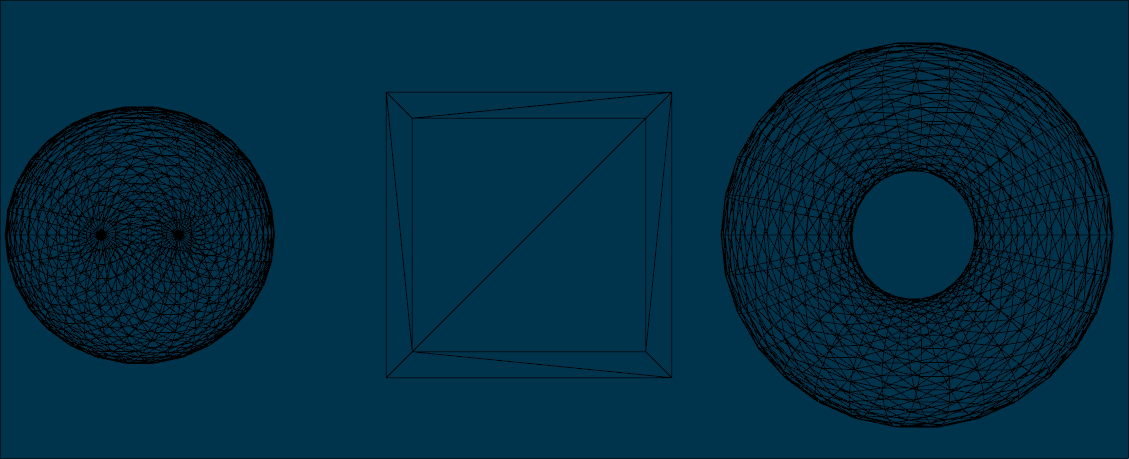
\includegraphics[width=.9\linewidth]{img/test14.png}
\caption{Prymitywy.}
\end{figure}

\begin{verbatim}
/**
 *@file
 *@brief Primitives example.
 **/

#include "cube.hpp"
#include "engine.hpp"
#include "light.hpp"
#include "sphere.hpp"
#include "torus.hpp"

/// engine reference
Engine &engine{Engine::getInstance()};

int main() {
  /// Set ProjectionType perspective so that it looks natural.
  engine.setProjectionType(Engine::ProjectionType::perspective);

  // Enable wireframe mode so that shapes can be noticed
  engine.setWireframeMode(true);

  /// Instanitate Cube
  Cube *cube{new Cube{}};
  // Set Cube position
  cube->setPosition(0, 0, -10);
  /// Add cube to engine
  engine.addDrawable(cube);

  /// Add Sphere
  Sphere *sphere{new Sphere{}};
  sphere->setPosition(-3, 0, -10);
  engine.addDrawable(sphere);

  /// Add torus
  Torus *torus{new Torus{}};
  torus->setScale(0.5);
  torus->setPosition(3, 0, -10);
  engine.addDrawable(torus);

  /// activate loop
  engine.loop();
}
\end{verbatim}
\subsection{Teksturowanie}
\label{sec:org9cb56de}

\begin{figure}[htbp]
\centering
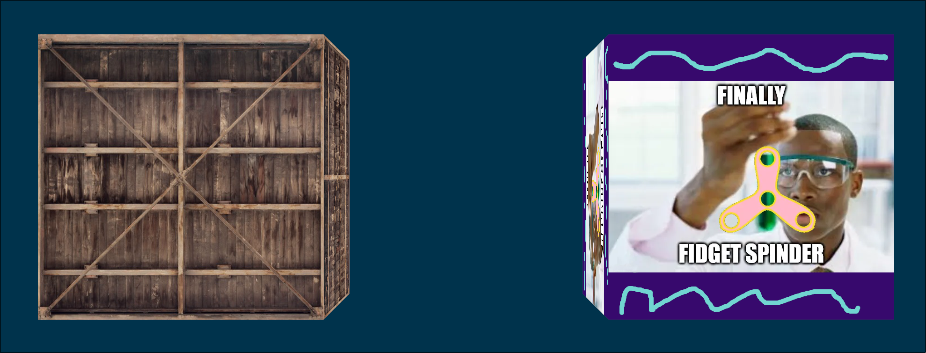
\includegraphics[width=.9\linewidth]{img/test15.png}
\caption{Teksturowanie obiektów.}
\end{figure}

\begin{verbatim}
/**
 *@file
 *@brief Textures example.
 **/

#include "cube.hpp"
#include "engine.hpp"

/// engine reference
Engine &engine{Engine::getInstance()};

int main() {
  /// Set ProjectionType perspective so that it looks natural.
  engine.setProjectionType(Engine::ProjectionType::perspective);

  /// Add light to engine that is full ambient light so that textures are
  /// visible
  Light *light{new Light{}};
  light->setAmbient(glm::vec3{1});
  engine.addLight(light);

  /// Instanitate Cube with diffuse light texture
  Cube *cube{new Cube{Texture{Texture::TextureType::diffuse,
                              getResourcesPath() + "textures/container.png"}}};
  // Set Cube position
  cube->setPosition(-2, 0, -10);
  /// Add cube to engine
  engine.addDrawable(cube);

  // Add another cube with another texture
  Cube *cube2{new Cube{Texture{Texture::TextureType::diffuse,
                               getResourcesPath() + "textures/eureka.png"}}};
  // flip the cube
  cube2->rotate(glm::radians(90.f), {1, 0, 0});
  cube2->setPosition(2, 0, -10);
  engine.addDrawable(cube2);

  /// activate loop
  engine.loop();
}
\end{verbatim}
\subsection{Oświetlenie, cieniowanie, transformacje}
\label{sec:org2fd61dc}

\begin{figure}[htbp]
\centering
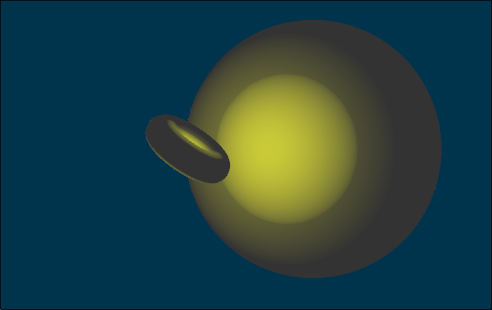
\includegraphics[width=.9\linewidth]{img/test16.png}
\caption{Środek pączka jest źródłem światła}
\end{figure}


\begin{verbatim}
/**
 *@file
 *@brief Light example.
 **/

#include "engine.hpp"
#include "sphere.hpp"
#include "torus.hpp"
#include <cmath>
#include <glm/fwd.hpp>
#include <glm/trigonometric.hpp>

/// engine reference
Engine &engine{Engine::getInstance()};

constexpr float rotateSpeed{10};
constexpr glm::vec3 rotationAxis{0, 1, 1};
constexpr float lightDistance{2};

int main() {
  /// Set ProjectionType perspective so that it looks natural.
  engine.setProjectionType(Engine::ProjectionType::perspective);

  /// Add light to engine that is full ambient light so that textures are
  /// visible
  Light *light{new Light{}};
  light->setAmbient(glm::vec3{0.2});
  constexpr glm::vec3 lightColor{0.3, 0.3, 0.01};
  light->setSpecular(lightColor);
  light->setDiffuse(lightColor);
  // move light up
  light->setPosition(0, 1, 0);
  engine.addLight(light);

  Shape *sun{new Torus{}};
  engine.addDrawable(sun);
  sun->setScale(0.1);

  // Add another cube with another texture
  Shape *ball{new Sphere{}};

  // flip the cube
  ball->rotate(glm::radians(90.f), {1, 0, 0});
  ball->setPosition(0, 0, -10);
  engine.addDrawable(ball);

  // Rotate the cubes
  engine.setLoopFunction([&]() {
    static float time{};
    float dt{engine.getLastFrameDuration().asSeconds()};

    time += dt;
    if (time > 2 * M_PI) {
      time -= 2 * M_PI;
    }

    float x{static_cast<float>(sin(time) * lightDistance)};
    float z{static_cast<float>(cos(time) * lightDistance)};

    sun->setPosition(glm::vec3{0, 0, -10} + glm::vec3{x, 0, z});
    light->setPosition(glm::vec3{0, 0, -10} + glm::vec3{x, 0, z});

    sun->rotate(rotateSpeed * dt, rotationAxis);

    // ball->rotate(glm::radians(cubeRotateSpeed * dt), cubeRotationAxis);
    //
  });

  /// activate loop
  engine.loop();
}
\end{verbatim}
\section{Wybrane testy}
\label{sec:org727f404}
\subsection{Test 10}
\label{sec:org011e1f8}

\begin{figure}[htbp]
\centering
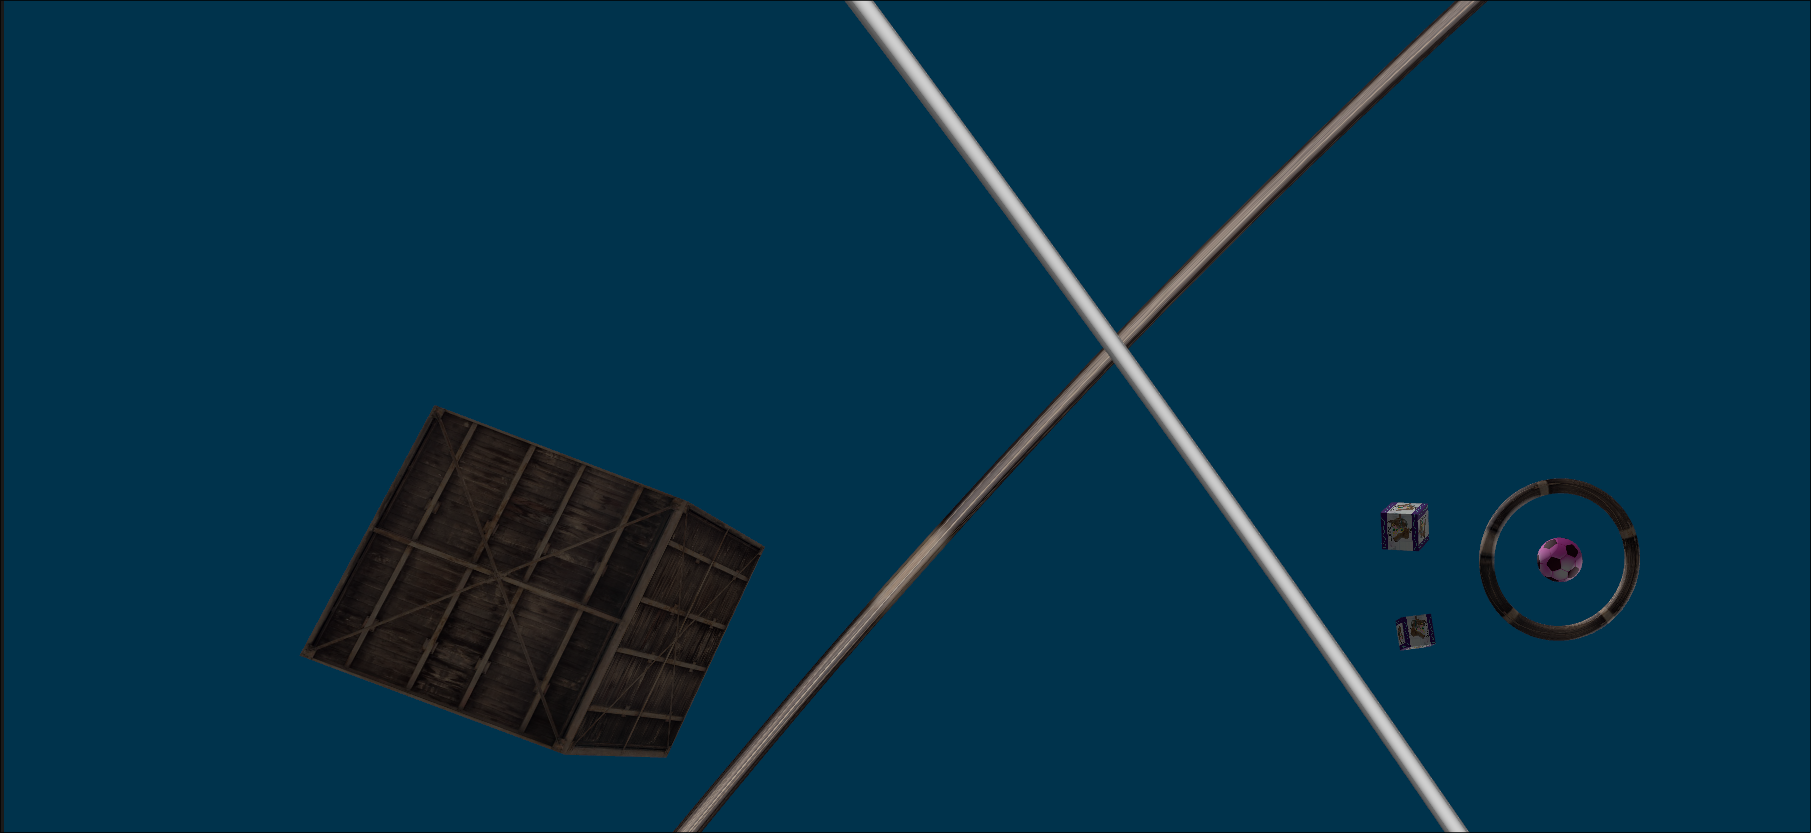
\includegraphics[width=.9\linewidth]{img/test10.png}
\caption{Zrzut ekranu z test10}
\end{figure}

\begin{verbatim}
/**
 *@file
 *@brief Test shapes.
 **/

#include "SFML/Window/Event.hpp"
#include "SFML/Window/Keyboard.hpp"
#include "cube.hpp"
#include "engine.hpp"
#include "light.hpp"
#include "resources.hpp"
#include "sphere.hpp"
#include "texture.hpp"
#include "torus.hpp"
#include <glm/fwd.hpp>

Engine &engine{Engine::getInstance()};

int main() {
  engine.setProjectionType(Engine::ProjectionType::perspective);
  engine.setCameraHandlingKeyboard(true);
  engine.setCameraHandlingMouse(true);
  engine.getWindow().setMouseCursorGrabbed(true);
  engine.getWindow().setMouseCursorVisible(false);

  engine.setEventHandler(Engine::Event::KeyReleased, [](sf::Event ev) {
    static bool wireOn{false};
    if (ev.key.code == sf::Keyboard::Key::M) {
      LOGINFO << "Switching wireframe mode " << wireOn << '\n';
      engine.setWireframeMode(wireOn = !wireOn);
    }
  });

  engine.setMaxFps(75);

  Shape *boxContainer =
      new Cube{Texture{Texture::TextureType::diffuse,
                       getResourcesPath() + "/textures/container.png"},
               Texture{Texture::TextureType::specular,
                       getResourcesPath() + "/textures/container.png"}};

  boxContainer->setPosition(-5, 0, 10);
  boxContainer->setScale(2);
  engine.addDrawable(boxContainer);

  Shape *boxMeme =
      new Cube(Texture{Texture::TextureType::diffuse,
                       getResourcesPath() + "/textures/eureka.png"});
  engine.addDrawable(boxMeme);
  boxMeme->setPosition(0, -1, -3);
  boxMeme->setScale(0.2);

  Shape *boxMemeFast =
      new Cube(Texture{Texture::TextureType::diffuse,
                       getResourcesPath() + "/textures/eureka.png"});
  boxMemeFast->setPosition(-3, 1, -3.5);
  boxMemeFast->setScale(0.3);
  engine.addDrawable(boxMemeFast);

  Shape *ball =
      new Sphere(1, Texture{Texture::TextureType::diffuse,
                            getResourcesPath() + "/textures/ball.png"});
  engine.addDrawable(ball);
  ball->setScale(0.3);

  Shape *paczek{new Torus(0.1, 1,
                          {Texture::TextureType::diffuse,
                           getResourcesPath() + "textures/container.png"},
                          {Texture::TextureType::specular}, 80, 80)};

  engine.addDrawable(paczek);

  ball->setPosition({0, 0, -5});
  paczek->setPosition({0, 0, -5});

  Shape *gigaPaczek{new Torus(0.3, 25,
                              {Texture::TextureType::diffuse,
                               getResourcesPath() + "textures/container.png"},
                              {Texture::TextureType::specular},
                              Torus::s_defaultSidesCount, 100)};

  engine.addDrawable(gigaPaczek);

  Shape *gigaPaczek2{new Torus(0.3, 24,
                               {
                                   Texture::TextureType::diffuse,
                               },
                               {Texture::TextureType::specular}, 30, 100)};

  engine.addDrawable(gigaPaczek2);

  ball->setPosition({0, 0, -5});
  paczek->setPosition({0, 0, -5});

  Shape *lightCube{new Cube{}};
  engine.addDrawable(lightCube);
  lightCube->setScale(0.1);
  lightCube->setPosition(0, 15, 0);

  Light *light{new Light{}};
  light->setAmbient(glm::vec3{0.3});
  light->setDiffuse(glm::vec3{0.25});
  light->setSpecular({0.3, 0.3, 0.3});

  light->setPosition({0, 15, 0});

  engine.addLight(light);

  engine.setLoopFunction([&]() {
    engine.moveMouseToCenterOfWindow();
    static constexpr float angleSpeed{60};

    const float rotation{
        glm::radians(angleSpeed * engine.getLastFrameDuration().asSeconds())};

    paczek->rotate(rotation * 0.3, {1, 0, 1});
    gigaPaczek->rotate(rotation * 0.10, {-1, 1, 1});
    gigaPaczek2->rotate(rotation * 0.10, {1, 0, -1});
    ball->rotate(rotation, {-0.5, 1, 0});
    boxContainer->rotate(rotation * 0.3, {1, 0, 0});
    boxMeme->rotate(rotation, {-1, 0, 0});
    boxMemeFast->rotate(rotation * 5, {0, 0.5, 0.5});
  });

  engine.loop();
}
\end{verbatim}
\subsection{Test 11}
\label{sec:orgd35187e}

\begin{figure}[htbp]
\centering
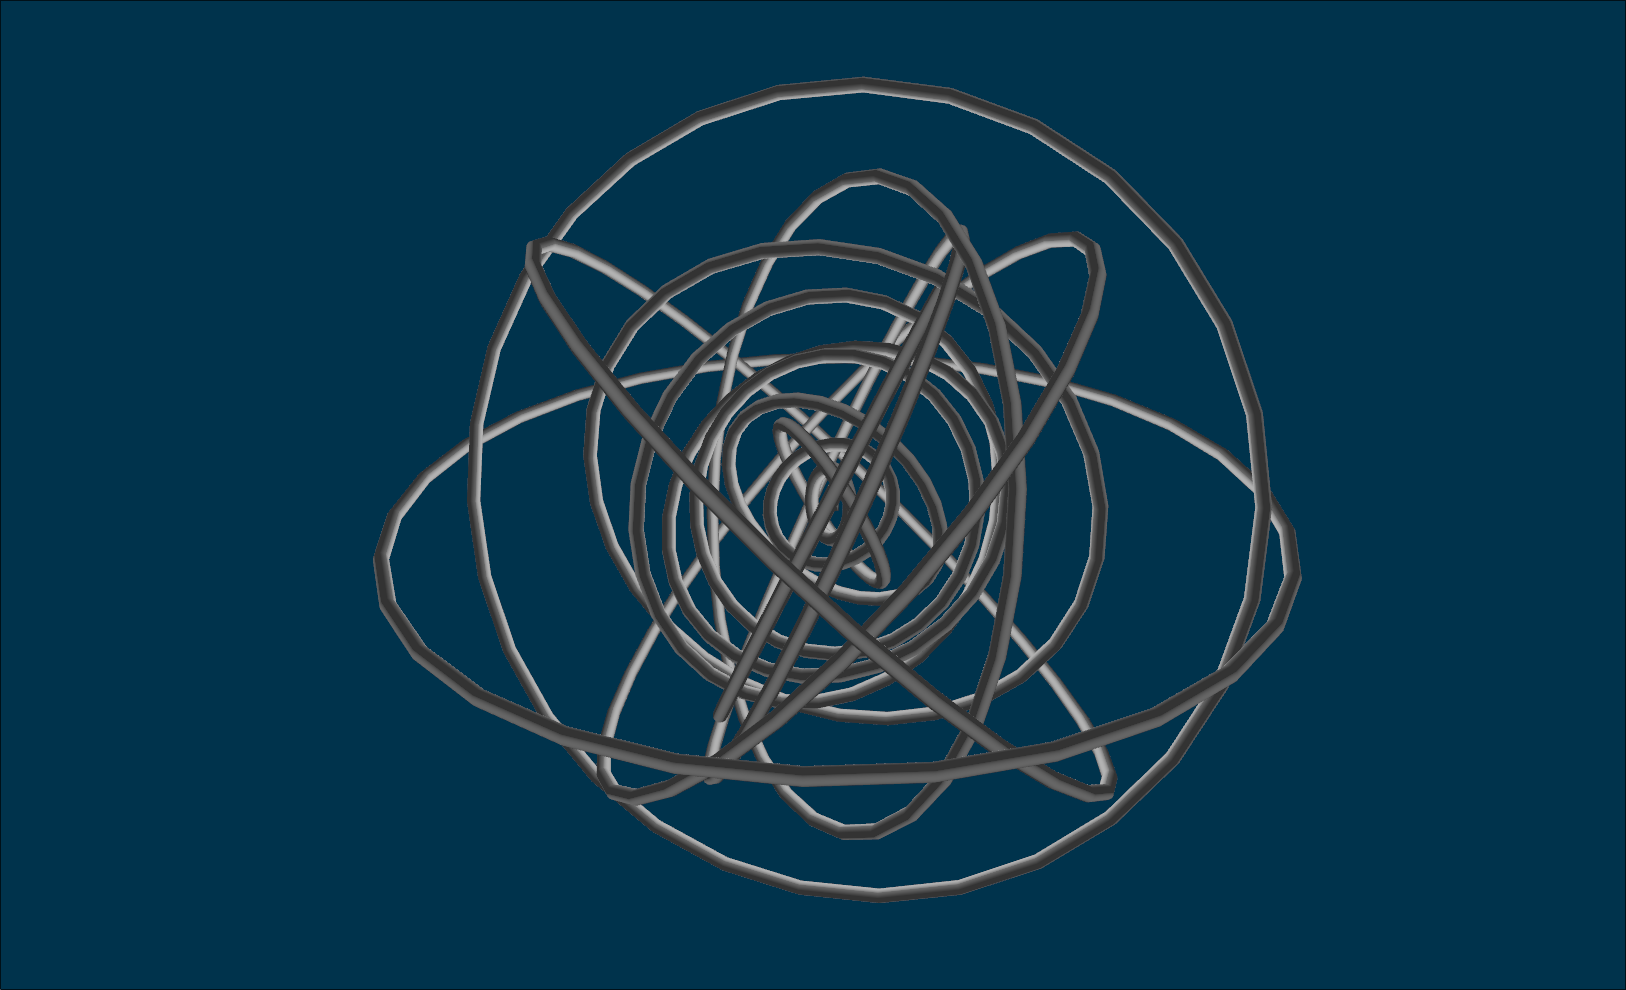
\includegraphics[width=.9\linewidth]{img/test11.png}
\caption{Zrzut ekranu z test11}
\end{figure}


\begin{verbatim}
#include "cube.hpp"
#include "drawable.hpp"
#include "engine.hpp"
#include "light.hpp"
#include "log.hpp"
#include "shape.hpp"
#include "time.h"
#include "torus.hpp"
#include <cstdlib>
#include <glm/fwd.hpp>
#include <iostream>
#include <random>

Engine &engine{Engine::getInstance()};

constexpr int paczekcount{15};
constexpr float paczekRotationSpeed{15};

constexpr float rotationChangeIntervalSeconds{2};

void init() {
  engine.setProjectionType(Engine::ProjectionType::perspective);
  engine.setCameraHandlingKeyboard(true);
  engine.setCameraHandlingMouse(true);
  engine.getWindow().setMouseCursorGrabbed(true);
  engine.getWindow().setMouseCursorVisible(false);

  engine.setEventHandler(Engine::Event::KeyReleased, [](sf::Event ev) {
    static bool wireOn{false};
    if (ev.key.code == sf::Keyboard::Key::M) {
      LOGINFO << "Switching wireframe mode " << wireOn << '\n';
      engine.setWireframeMode(wireOn = !wireOn);
    }
  });
}

int main() {
  init();

  Light *light{new Light{}};
  engine.addLight(light);

  light->setAmbient(glm::vec3{0.2});
  light->setDiffuse(glm::vec3{0.3});
  light->setSpecular(glm::vec3{0.2});

  Cube *lightBox{new Cube};
  engine.addDrawable(lightBox);

  light->setPosition({0, 0, 0});
  lightBox->setPosition({0, 0, 0});
  lightBox->setScale(glm::vec3{0.1});

  std::vector<Shape *> paczki;

  for (int i{}; i < paczekcount; ++i) {
    Shape *tmp{new Torus{static_cast<float>(0.1),
                         static_cast<float>(0.5 + 0.2 * (i * 2))}};
    paczki.push_back(tmp);
    engine.addDrawable(tmp);
  }

  srand(time(0));

  std::random_device rd;
  std::default_random_engine randEng(rd());
  std::uniform_real_distribution<float> dist(0, 1);

  glm::vec3 rotationVector[paczekcount];

  for (glm::vec3 &i : rotationVector) {
    i = {dist(rd), dist(rd), dist(rd)};
  }

  float dt{};

  engine.setLoopFunction([&]() {
    engine.moveMouseToCenterOfWindow();

    dt += engine.getLastFrameDuration().asSeconds();
    if (dt > rotationChangeIntervalSeconds) {
      dt = 0;
      for (glm::vec3 &i : rotationVector) {
        i = {dist(rd), dist(rd), dist(rd)};
      }
    }
    for (int i{}; i < paczekcount; ++i) {
      paczki[i]->rotate(glm::radians((paczekcount - i + 1) *
                                     engine.getLastFrameDuration().asSeconds() *
                                     paczekRotationSpeed),
                        glm::vec3{rotationVector[i]});
    }
  });

  engine.loop();
}
\end{verbatim}
\end{document}